\section{KKT podmínky}
\subsection{Věta o nutných KKT podmínkách}\label{KKT}
Nechť $\Omega \subseteq \R^n$ je otevřená množina, $f, g_1, \dots, g_k \in C^1 (\Omega)$,
\[
  M = \bc{x \in \Omega \mid g_1(x) \leq 0, \dots, g_k(x) \leq 0} \text{ a } \hat{x}\in M.
\]
Jestliže $\overline{\F(M; \hat x)} = \G(\hat x)$ a $\hat x$ je bod lokálního minima na $f$ na $M$, 
pak existuje ${(\mu_1, \dots, \mu_k)^T \in \R^k}$ tak, že 
\begin{align*}
    \nabla f(\hat x) + \Sigma_{i=1}^k \mu_i \nabla g_i(\hat x) &= 0, \\
    \mu_i g_i(\hat x) &= 0 \text{ pro všechna } i \in \bc{1, \dots, k}, \\
    \mu_i &\geq 0 \text{ pro všechna } i \in \bc{1, \dots, k}.
\end{align*}

Důkaz.

\begin{itemize}
    \item $\I(\hat x) = \emptyset \implies \hat x \in \Int(M) \implies \nabla f(\hat x) = 0$ z 
    \hyperref[fermat]{Fermatovy věty}. \\
    $\rightarrow$ volba $\mu_1 = \dots = \mu_k = 0$. Pak KKT podmínky splněny.
    \item $\emptyset \not= \I(\hat x) = \bc{1, \dots, l}$\\
    Víme, že máme bod lokálního minima ($\hat x$) $\underset{\text{\hyperref[fermat]{věta}}}
    {\overset{\text{\hyperref[fermat]{Fermatova}}}{\implies}} \F(M; \hat x) \cap \D_0(f; \hat x) = \emptyset$, \\
    tj. $\langle \nabla f(\hat x), d\rangle \geq 0 \quad \forall d \in \F(M; \hat x)$. 

    Teď chceme dokázat, že platí $\langle \nabla f(\hat x), d\rangle \geq 0 \quad \forall d \in \G(\hat x)$. 

    Protože $\overline{\F(M; \hat x)}$ koinciduje s $\G(\hat x)$ a ze spojitosti skalárního součinu plyne, že \\ 
    $\langle \nabla f(\hat x), d\rangle \geq 0 \quad \forall d \in \underbrace{\overline{\F(M; \hat x)}}_{\G(\hat x)}$.

    To tedy znamená $\langle \nabla f(\hat x), d\rangle \geq 0 \quad \forall d \in \G(\hat x)$. Z toho plyne, že
    neexistuje $d \in \R^n$, pro který platí:
    \begin{equation*}
        \settowidth{\mylen}{$\displaystyle \langle \nabla g_1(\hat x), d \rangle \leq {}$\,}
        \begin{aligned}
            \langle \nabla f(\hat x), d \rangle &< 0 \, \dots \text{ tj. } \langle -\nabla f(\hat x), d\rangle > 0 \\
            &\phantom{{}<{}}
            \hspace*{-\dimexpr\mylen+\nulldelimiterspace}
              \left.\begin{aligned}
                  \langle \nabla g_1(\hat x), d \rangle &\leq 0 \\
                  & \vdots \\
                  \langle \nabla g_l(\hat x), d \rangle &\leq 0
              \end{aligned}\right\}
              A^T d \leq 0, \text{ kde } A = (\nabla g_1(\hat x), \dots, \nabla g_l(\hat x))
        \end{aligned}
    \end{equation*}
    No a z \hyperref[farkas]{Farkasova lemma} tedy nutně platí: ex. $\mu = (\mu_1, \dots, \mu_l)^T \in \R^l_+ : 
    \underbrace{A \mu}_{\hspace*{-2em}\sum_{i=1}^l \mu_i \nabla g_i} = - \nabla f(\hat x)$.\\
    $\rightarrow$ volme dále $\mu_{l+1}, \dots, \mu_k = 0$. Pak
    \begin{align*}
        - \nabla f(\hat x) &= \sum_{i=1}^k \mu_i \nabla g_i(\hat x), \\
        \mu_i \nabla g_i(\hat x) &= 0 \text{ pro všechna } i \in \bc{1, \dots, k}, \\
        \mu_i &\geq 0 \text{ pro všechna } i \in \bc{1, \dots, k}.
    \end{align*}
    A to jsou přesně KKT podmínky. $\qed$
\end{itemize}

\subsection{Terminologie KKT podmínek}
\begin{itemize}
    \item Podmínky
    \begin{align*}
        &(\text{P}1) \: \nabla f(\hat x) + \sum_{i=1}^{k}\mu_i \nabla g_i(\hat x) = 0, \\
        &(\text{P}2) \: \mu_i g_i(\hat x) = 0, \\
        &(\text{P}3) \: \mu_i \geq 0,
    \end{align*}
    se souhrně nazývají \bb{KKT podmínky}.
    \item Podmínka (P1) se nazývá \bb{podmínka stacionarity}.
    \item Podmínka (P2) se nazývá \bb{podmínka komplementarity}.
    \item Koeficienty $\mu_1, \dots, \mu_k \in \R$ splňující KKT podmínky se nazývají \bb{KKT multiplikátory} 
    \\ (Lagrangeovy multiplikátory) v bodě $\hat x$.
    \item Bod $\hat x$ se nazve \bb{KKT bod}, existuje-li vektor $(\mu_1, \dots, \mu_k)^T$ KKT multiplikátorů v bodě 
    $\hat x$.
\end{itemize}

\subsection{Příklad použití KKT podmínek}
\Opt{min}{}{\underbrace{x + y}_{f(x,y)}}{
    \underbrace{x}_{g_1(x,y)} \: &\geq 0, \\
    \underbrace{y}_{g_2(x,y)} \: &\geq 0.
}
Určete KKT body.\\
$\nabla f(x, y) = 
\begin{bmatrix}
    1 \\
    1
\end{bmatrix}$, $\nabla g_1(x,y) = 
\begin{bmatrix}
    -1 \\
    \phantom{-}0
\end{bmatrix}$, $\nabla g_2(x,y) = 
\begin{bmatrix}
    \phantom{-}0 \\
    -1
\end{bmatrix}$.

KKT podmínky:
\begin{align*}
    1 + \mu_1 (-1) + \mu_2 (0)  &= 0 \quad \rightarrow \mu_1 = 1 \\
    1 + \mu_1 (0) +  \mu_2 (-1) &= 0 \quad \rightarrow \mu_2 = 1 \\
    \mu_1 (-x) &= 0 \\
    \mu_2 (-y) &= 0 \\
    \mu_1, \mu_2 &\geq 0
\end{align*}
Jediný KKT bod je tedy 
$\hat x = \begin{bmatrix}
    0 \\
    0
\end{bmatrix}$ a jedná se o bod minima.

\subsection{Příklad, že KKT podmínky vždy nenaleznou všechny body}
\Opt{min}{}{x}{
    x^2 + (y-1)^2 \: &\leq 1, \\
    x^2 + (y+1)^2 \: &\leq 1.
}
\begin{multicols}{2}
    Nákres.
    \hspace{2em}
    \begin{figure}[H]
        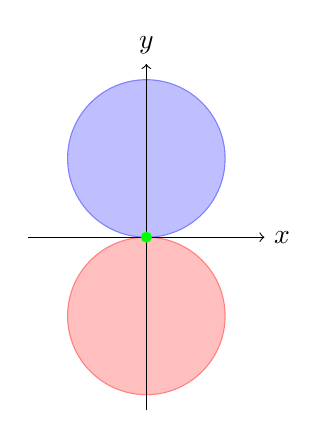
\begin{tikzpicture}[scale=1]
            \fill[blue!50, opacity=0.5] (0,1) circle (1);
            \fill[red!50, opacity=0.5] (0,-1) circle (1);
            
            \draw[blue!50] (0,1) circle (1);
            \draw[red!50] (0,-1) circle (1);
            
            \draw[->] (-1.5,0) -- (1.5,0) node[right] {$x$};
            \draw[->] (0,-2.2) -- (0,2.2) node[above] {$y$};

            \fill[green] (0,0) circle (2pt);
        \end{tikzpicture}
    \end{figure}

\columnbreak

    \textcolor{green}{Přípustná} množina: $M = \bc{0} \rightarrow$ určitě konvexní množina.

    KKT podmínky: 
    \begin{align*}
        1 + \mu_1 (2 \cdot 0) &+ \mu_2 (2 \cdot 0) = 0 \, \xmark \\
        &\vdots
    \end{align*}
    $\Rightarrow (0,0)$ není KKT bod i když je úloha konvexní a bod $(0,0)$ je očividně bodem minima.
\end{multicols}

\subsection{Afinní podmínka regularity}\label{afinniPodm}
Nechť $\Omega \subseteq \R^n$ je otevřená množina, $g_1, \dots, g_k \in C^1 (\Omega)$ a 
\[
    M = \bc{x \in \Omega \mid g_1(x) \leq 0, \dots, g_k(x) \leq 0}.
\]
Řekněme, že $(g_i)_{i=1}^k$ splňuje afinní podmínku regularity, jestliže $g_1, \dots, g_k$ jsou afinní.

\subsection{Slaterova podmínka regularity}\label{slaterPodm}
Nechť $\Omega \subseteq \R^n$ je otevřená množina, $g_1, \dots, g_k \in C^1 (\Omega)$ a 
\[
    M = \bc{x \in \Omega \mid g_1(x) \leq 0, \dots, g_k(x) \leq 0}.
\]
Řekněme, že $(g_i)_{i=1}^k$ splňuje Slaterovu podmínku regularity, jestliže $g_1, \dots, g_k$ jsou konvexní na $\Omega$
a existuje $x \in \Omega$ tak, že pro každé $i \in \bc{1, \dots, k}$ je $g_i(x) < 0$.

\subsection{Věta o postačujících KKT podmínkách}
Nechť $\Omega \subseteq \R^n$ je otevřená množina, $f, g_1, \dots, g_k \in C^1(\Omega)$ jsou konvexní funkce na \\
$C = \bc{x \in \Omega \mid g_1(x) \leq 0, \dots, g_k(x) \leq 0}$. Jestliže $\hat x \in C$ je KKT bod, pak $\hat x$ je 
bod minima funkce $f$ na $C$.

Důkaz. Ať $x \in C$. \\
Cíl: $f(x) - f(\hat x) \geq 0$ ($= \hat x$ je minimum)

Charakterisace pomocí tečné nadroviny: $f(\hat x) + \langle \nabla f(\hat x), x - \hat x\rangle \leq f(x) \quad x, 
\hat x \in C$
\[
    f(x) - f(\hat x) \underset{\substack{\text{$f$ je konvexní } \\ \text{na $C \subseteq \Omega$}} }{\geq} \langle 
    \nabla f(\hat x), x - \hat x\rangle \underset{\text{stacionarity}}{\overset{\text{podmínka}}{=}} 
    \langle - \sum_{i=1}^{k} \mu_i \nabla g_i(\hat x), x - \hat x\rangle
\]
\[
    = \sum_{i=1}^{k} - \langle \nabla g_i(\hat x), x - \hat x \rangle \mu_i = \sum_{i=1}^{n} (g_i(\hat x) - g_i(x)) \mu_i 
    \underset{\text{komplementarity}}{\overset{\text{podmínka}}{=}} - \sum_{i=1}^{n}    
    \underbrace{\mu_i}_{\substack{\text{podmínka}\\ \text{nezápornosti}}} \overbrace{g_i(x)}^{\leq 0 \, \forall x \in C}
    \geq 0. \qed
\]
\newpage
\subsection{Použití podmínek regularity k ověření KKT podmínek}
\begin{multicols}{2}
    \Opt{min}{}{2x^2 + y^2}{
        x^2 + y^2 - 1 \: &\leq 0, \\
        -x \: &\leq 0.
    }
    \hyperref[afinniPodm]{Afinní podmínka} splněna není, \\ ověříme \hyperref[slaterPodm]{Slaterovu}.

\columnbreak

    \begin{figure}[H]
        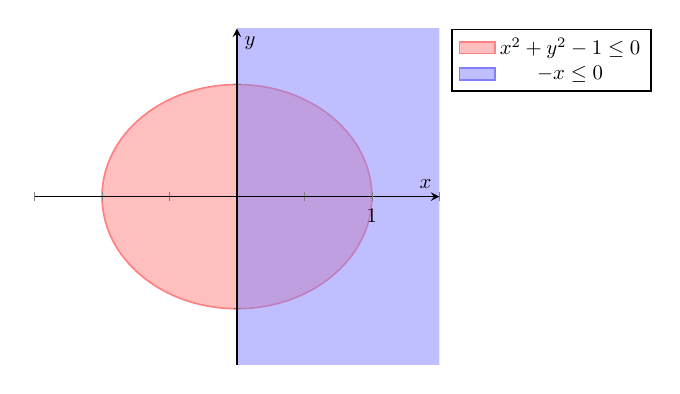
\begin{tikzpicture}[scale=0.75]
            \begin{axis}[
            axis lines=middle,
            axis on top,
            xlabel={$x$},
            ylabel={$y$},
            xmin=-1.5, xmax=1.5,
            ymin=-1.5, ymax=1.5,
            thick,
            xticklabels={},
            yticklabels={},
            extra x ticks={1},
            %legend pos=north west,
            %legend style={nodes={scale=0.5, transform shape}},
            legend pos=outer north east,
            ]
            \fill[red!50, opacity=0.5] (0,0) circle (1);
            \draw[red!50] (0,0) circle (1);
            \addlegendimage{area legend,red!50,fill=red!50,fill opacity=0.5}
            \fill[blue!50, opacity=0.5] (0,-2.5) rectangle (2.5,2.5);
            \addlegendimage{area legend,blue!50,fill=blue!50,fill opacity=0.5}
            \addlegendentry{$x^2+y^2-1\leq0$}
            \addlegendentry{$-x\leq0$}
            \end{axis}
        \end{tikzpicture}
    \end{figure}
\end{multicols}

Množina je očividně konvexní a zároveň zvolme $x = 
\begin{bmatrix}
    \frac{1}{2} \\
    0    
\end{bmatrix} \in \Omega$. Pak $g_i (x) < 0$, Slaterova podmínka je tedy očividně splněna.

$\nabla f (x) = 
\begin{bmatrix}
    4x \\
    2y    
\end{bmatrix}, \nabla g_1(x) =
\begin{bmatrix}
    2x \\
    2y
\end{bmatrix}, \nabla g_2(x) = 
\begin{bmatrix}
    -1\\
    \phantom{-}0
\end{bmatrix}$.

$\implies$ KKT podmínky:
\begin{align*}
    4x + \mu_1 2 x + \mu_2 (-1) &= 0 \leftrightarrow 2x (2+\mu_1) - \mu_2 = 0 \\
    2y + \mu_1 2 y + \mu_2 0    &= 0 \Leftrightarrow 2y (1+\mu_1) = 0 \underset{\mu_1 \geq 0}{\implies} y = 0 \\
    \mu_1(x^2 + y^2 - 1) &= 0 \\
    \mu_2(-x) &= 0 \\
    \mu_1, \mu_2 &\geq 0  
\end{align*}

$y=0$:
\[
    \begin{rcases*}
        2x(2+ \mu_1) = \mu_2 \\
        \mu_1(x^2 + 1) = 0 \\
        \mu_2 x = 0 \\
        \mu_1, \mu_2 \geq 0
    \end{rcases*}
    \begin{aligned}
        &x \not= 0 \Rightarrow \mu_2 = 0 \Rightarrow 2 + \mu_1 = 0 \dots \text{ spor s } \mu_1 \geq 0.\\
        &x = 0 \Rightarrow \mu_1 = 0 \Rightarrow \mu_2 = 0 \quad \checkmark
    \end{aligned}
\]

Existuje bod $
\begin{bmatrix}
x \\
y    
\end{bmatrix} =
\begin{bmatrix}
    0 \\
    0
\end{bmatrix}$, pro který jsou splněny nutné a postačující KKT podmínky.

\subsection{Určení nutných a postačujících podmínek optimality}
Ať $A \in \M_{m,n} (\R), \, D \in \M_{r,n}(\R), \, b\in \R^m$ a $\lambda > 0$. Je dána úloha
\[
    \text{minimalisujte } f(x) = \| Ax - b\|^2 + \lambda \| Dx\|^2  \text{ na } \R^n.
\]
Jaké jsou nutné a postačující podmínky optimality?
\begin{align*}
    f(x) &= \langle Ax - b, Ax - b\rangle + \lambda \langle Dx, Dx\rangle \\
    &= \langle \underbrace{Ax, Ax}_{A^TAx, x}\rangle - 2\langle Ax, b\rangle + \| b\|^2 + \lambda \langle 
        \underbrace{Dx, Dx}_{D^TDx, x}\rangle
\end{align*}
$\implies f(x) = \left\langle \left(A^TA + \lambda D^TD\right)x, x\right\rangle - 2 \left\langle x, A^T b\right\rangle 
+ \| b\|^2$\\
Je $f$ konvexní?\\
Ano, neboť $\nabla^2 f(x) = 2(A^TA + \lambda D^TD)$ je positivně semidefinitní, protože pro $x \in \R$:
\begin{align*}
    \left\langle 2\left(A^TA + \lambda D^TD\right)x, x\right\rangle &= 2 \left[ \langle Ax, Ax\rangle + \lambda 
    \langle Dx, Dx\rangle\right] \\
    &= 2 \left[ \|Ax\|^2 + \lambda \|Dx\|^2\right] \geq 0
\end{align*}
Tedy $f$ je konvexní $\implies$ stačí najít stacionární body.
\begin{align*}
    0 = \nabla^2 f(x) &= 2 (A^TA + \lambda D^TD)x - 2(A^Tb) + 0 \\
    &= (A^TA + \lambda D^TD)x - A^Tb
\end{align*}
\[
    \implies A^Tb = (A^TA + \lambda D^TD)x
\]
A to je nutná a postačující podmínka pro $x$, aby byl bodem minima $f$ na $\R^n$.
    
\subsection{Určení KKT podmínek}
\Opt{min}{}{x^4 + y^4 + 12 x^2 + 6 y^2 - xy - x - y}{
    x + y \: &\geq 6, \\
    2x-y \: &\geq 3, \\
    x, y \: &\geq 0.
}
\begin{enumerate}[(a)]
    \item Napište KKT podmínky.
    \item Jsou nutné a postačující?
    \item Ukažte, že $(3, 3)^T$ je jediný bod minima.
\end{enumerate}
(a) Mějme
\begin{align*}
    g_1(x,y) &= -x-y+6, \\
    g_2(x,y) &= 2x-y+3, \\
    g_3(x,y) &= -x, \\
    g_4(x,y) &= -y, \\
    f(x,y) &= x^4 + y^4 + 12 x^2 + 6 y^2 - xy - x - y.
\end{align*}
$\rightarrow$ použijeme \hyperref[afinniPodm]{afinní podmínku regularity} $\rightarrow g_i$ jsou affiní.

KKT podmínky: 
\begin{align*}
    \nabla f(x, y) + \mu_1 \nabla g_1(x, y) + \mu_2 \nabla g_2(x, y) + \mu_3 \nabla g_3(x, y) + \mu_4 \nabla g_4(x, y) = 0 \\
    \mu_i g_i (x,y) = 0, i = 1,2,\dots,\\
    \mu_i \geq 0, i = 1,2,\dots.
\end{align*}
Tedy:
\begin{align*}
    4x^3 + 24x - y - 1 - \mu_1 - 2\mu_2 - \mu_3 = 0\phantom{,} \\
    4y^3 + 12y - x - 1 - \mu_1 + \mu_2 - \mu_4 = 0\phantom{,} \\
    \mu_1(-x-y+6) = 0, \\
    \mu_2(x-2y+3) = 0, \\
    x \mu_3 = 0, \\
    y \mu_4 = 0, \\
    \mu_1, \mu_2, \mu_3, \mu_4 \geq 0.
\end{align*}
Jsou postačující? Máme konvexní úlohu? Musíme ověřit konvexitu u $g_i$ a $f$.
\begin{itemize}
    \item $g_i$ jsou afinní $\implies$ jsou konvexní.
    \item $f:$
    \begin{itemize}
        \item kvadráty jsou ryze konvexní
        \item součet ryzích konvexních je ryzí konvexní
    \end{itemize} 
\end{itemize}
\[h(x, y) = 12x^2 + 6y^2 - xy -x -y\]
\[
    \nabla^2 h (x, y) = 
    \begin{bmatrix}
        \phantom{-}24 & -1 \\
        -1 & \phantom{-}12
    \end{bmatrix} = 24 \cdot 12 - 1 > 0; \quad 24 > 0 \implies h(x, y)\text{ je positivně definitní.}
\]
$\implies h(x, y)$ je ryze konvexní.

A proto je i $f(x, y)$ ryze konvexní, protože součet ryze konvexních dává ryze konvexní $\implies$ existuje právě jeden 
bod minima.\\
Ověříme $\begin{bmatrix} 3 \\ 3 \end{bmatrix}$. Ať $x=y=3$. Pak
\begin{align*}
    4 \cdot 27 + 24 \cdot 3 - 4 - \mu_1 + \mu_2 - \mu_3 = 0& \quad \text{(I.)} \\
    4 \cdot + 12 \cdot 3 - 4 - \mu_1 - 2\mu_2 - \mu_4 = 0& \quad \text{(II.)}\\
    \mu_1 \cdot 0 = 0& \\
    \mu_2 \cdot 0 = 0& \\
    3 \mu_3 = 0& \implies \mu_3 = 0\\
    3 \mu_4 = 0& \implies \mu_4 = 0\\
    \mu_1, \mu_2 \geq 0&
\end{align*}
I. $-$ II.: $24 \cdot 3 - 12 \cdot 3 - 3 \mu_2 = 0 \implies \mu_2 = \frac{1}{3} (24 \cdot 3 - 12 \cdot 3) > 0$.\\
$\mu_1 = 4 \cdot 27 + 24 \cdot 3 - 4 - \frac{2}{3}(24 \cdot 3 - 36) > 0$.

\subsection{Určení KKT podmínek}
\Opt{min}{}{\alpha x + y, \: \alpha \in \R \text{ je parametr.}}{
    x^2 + y^2 - 25 \: &\leq 0, \\
    x-y-1 \: &\leq 0.
}
Určete $\alpha$ tak, aby 
$\begin{bmatrix}
    4 \\
    3
\end{bmatrix}$ bylo řešení.

KKT podmínky:
\begin{align*}
    \alpha + \mu_1 (2x) + \mu_2 \cdot 1 = 0\phantom{,} \\
    1 + \mu_1 (2y) - \mu_2 = 0\phantom{,} \\
    \mu_1(x^2 + y^2 - 25) = 0, \\
    \mu_2(x - y - 1) = 0, \\
    \mu_1, \mu_2 \geq 0.
\end{align*}
$g_i$ jsou konvexní, $f$ je konvexní $\implies$ KKT podmínky jsou postačující.\\
\hyperref[slaterPodm]{Slaterova podmínka optimality} je splněna $\implies$ KKT podmínky jsou nutné.

$x=4, y=3$:
\begin{align*}
    \alpha + 8 \mu_1 + \mu_2 = 0& \quad \text{(I.)}\\
    1 + 6 \mu_1 - \mu_2 = 0&, \quad \text{(II.)}\\
    \mu_1, \mu_2 \geq 0&.
\end{align*}
I.+II.: $\alpha + 1 + 14 \mu_1 = 0$\\
$\mu_1 = \frac{-\alpha - 1}{14} \overset{!}{\geq} 0 \implies -1 \geq \alpha$. A tedy $\mu_2 = 1 + 6 \mu_1 \geq 0$.

Tedy aby
$\begin{bmatrix}
    4 \\
    3
\end{bmatrix}$ bylo řešení této úlohy, musí platit $\alpha \leq -1$.

\subsection{Určení KKT podmínek s trikem}
Mějme zadání
\Opt{min}{}{\frac{x_1}{x_2}}{
    \frac{1}{x_1} + x_2 \: &\leq 2, \\
    x_1, x_2 \: &> 0. 
}

\begin{multicols}{2}
    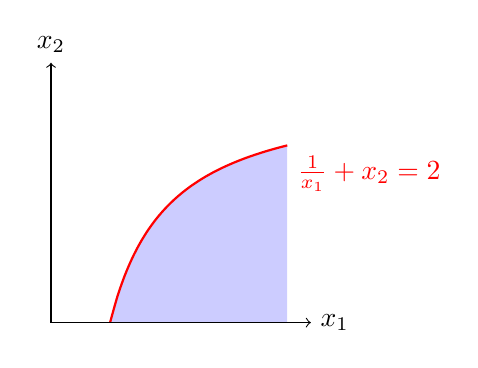
\begin{tikzpicture}[scale=1.5]
        \begin{scope}
            \clip (0,0) rectangle (2,2);
            \fill[blue!20] plot[domain=0.1:2] (\x, {2 - 1/(\x)}) -- (2,0) -- (0.1,0) -- cycle;
          \end{scope}
    
        \draw[domain=0.5:2, smooth, thick, red] 
          plot(\x, {2 - 1/(\x)})
          node[below right] {$\frac{1}{x_1} + x_2 = 2$};
    
        \draw[->] (0,0) -- (2.2,0) node[right] {$x_1$};
        \draw[->] (0,0) -- (0,2.2) node[above] {$x_2$};
    \end{tikzpicture}

\columnbreak

    Z nákresu množina vypadá konvexní, co ale minimalisovaná funkce?
    \[
        \nabla^2 f(x_1, x_2) = 
        \begin{bmatrix}
            0 & -\frac{1}{x^2_2} \\
            -\frac{1}{x^2_2} & \frac{2x_1}{x^3_2}    
        \end{bmatrix}
    \]
    \[
        \det \nabla^2 f(x_1, x_2) = -\frac{1}{x^4_2} < 0 \dots \text{indefinitní}
    \]
    $\implies$ KKT podmínky jsou jen nutné, nikoliv postačující.
\end{multicols}
Využijeme trik, uděláme substituci: $x_1 = e^{y_1}$, $x_2 = e^{y_2}$ $\dots$ $\varphi(y_1, y_2) = (e^{y_1}, e^{y_2})$,
$\varphi(\hat y_1, \hat y_2) = (\hat x_1, \hat x_2)$.\\
A úlohu převedeme na:
\Opt{min}{}{e^{y_1} - e^{y_2}}{
    e^{-y_1} + e^{y_2} \: &\leq 2.
}
\begin{align*}
    e^{\hat y_1 - \hat y_2} &\leq e^{y_1 - y_2} \\
    \underbrace{\frac{e^{\hat y_1}}{e^{\hat y_2}}}_{f(\varphi(\hat y_1, \hat y_2))} &\leq 
    \underbrace{\frac{e^{y_1}}{e^{y_2}}}_{f(\varphi(y_1, y_2))} \\
    f(\hat x_1, \hat x_2) &\leq f(x_1, x_2) \quad \forall (x_1, x_2) \in M.
\end{align*}
\hyperref[slaterPodm]{Slaterova podmínka} je splněna $\rightarrow (y_1, y_2) = (1, 0)$.\\
$\implies$ KKT podmínky jsou nutné a postačující.
\begingroup
\setcounter{equation}{0}
\renewcommand{\theequation}{\Roman{equation}}
\begin{align}
    e^{y_1 - y_2} + \mu(-e^{-y_1}) &= 0 \\
    -e^{y_1 - y_2} + \mu e^{y_2} &= 0 \rightarrow \mu = \frac{e^{y_1 - y_2}}{e^{y_2}} = e^{y_1 - 2y_2} \\
    \mu(e^{-y_1} + e^{y_2} - 2) &= 0 \\
    \mu &\geq 0
\end{align}
\endgroup
Očividně $\mu \not= 0 \implies e^{-y_1} + e^{y_2} - 2 = 0$ (III).
\begin{align*}
    \text{Dosazení (II) do (I): } e^{y_1 - y_2} - e^{-2y_2} &= 0. \\
    e^{y_1 - y_2} &= e^{-2y_2} \\
    y_1 - y_2 &= -2y_2 \\
    y_1 &= -y_2
\end{align*}
Dosazením do (III) získáme $2e^{y_2} - 2 = 0 \Rightarrow e^{y_2} = 1 \Rightarrow y_2 = 0 = y_1$.\\
Jediný bod minima je $[0,0]^T$.

Teď zpětný chod na původní úlohu: $x_1 = e^0 = 1$, $x_2 = e^0 = 1$. 

Původní úloha má řešení $[1, 1]^T$.
